\documentclass[12pt, letterpaper]{article}
\usepackage[utf8]{inputenc}
\usepackage{caption}
\usepackage{subcaption}
\usepackage{tabularx}
\usepackage{graphicx}
\usepackage{listings}
\usepackage{xcolor}
\def\code#1{\texttt{#1}}
\graphicspath{{./Pictures/}}


\setlength{\parskip}{1em}

%Set up listing env

\usepackage{xparse}



\NewDocumentCommand{\codeword}{v}{\texttt{\textcolor{blue}{#1}}}

\lstset{language=C,keywordstyle={\bfseries \color{blue}}}

\lstset{language=C,keywordstyle={\bfseries \color{blue}}}



\begin{document}

\begin{titlepage}
	\begin{center}
        \vspace*{1cm}	
		\title{Vacuum Meshing Guide}
		\author{William Ellis}
		\date{February 2022}   
		\maketitle
	\end{center}
\end{titlepage}

\maketitle
\section{Introduction}
In a variety of finite element problems, areas of interest include not just to the geometry of a studied part, but to the space around it as well. Ideally a mesh of the surrounding region is created when generating the original mesh. In practise however this is not always done. Without a mesh of the surrounding region, any variables of interest cannot be solved for. This tool has been created to help generate a vacuum region around a meshed part that did not initially possess one. 

\subsection{Problem Statement}
This tool is designed to help users generate a meshes vacuum region around a pre-existing mesh. This meshed vacuum region must conform to the nodes and elements on the pre-existing mesh so that no hanging nodes are present. 

\subsection{LibMesh and libIGL}
REFERENCES

\section{How Does it Work?}
The generation of the vacuum mesh can be broken down into 3 main steps. Firstly the surface mesh of the original part must be found. Secondly a boundary mesh is generated to enclose the surface mesh of the original part.  With both the skinned mesh and the boundry mesh, a well defined vacuum region is now present. The third step is to generate mesh elements in this vacuum region, to create the vacuum mesh. Due to the fact that currently only tri/ tet elements are supported in this 

\subsection{Mesh Skinning}
Skinning is the first step necessary to generate the vacuum mesh. Skinning refers to retrieving the surface mesh of a pre-existing mesh. This step is necessary as the skinned mesh will be used to inform the tetrahedraliation process which elements/ nodes on the original part it must conform to.

The skinning algorithm is fairly straight forward. A loop is done over all the elements in the mesh, in which each face/edge of the element is checked to see if it has a neighbour. If the face/edge has no neighbor, then the local face ID is added to a list. This check is done for all the faces/edges. Once completed, the nodes belonging to all the faces/edges in the list are added to their own list, and the connectivity data of these faces/edges is stored in another list. The new skinned mesh is then constructed using the list of nodes and the stored connectivity data.

\begin{figure}[ht]
	\begin{subfigure}{0.4\textwidth}
	    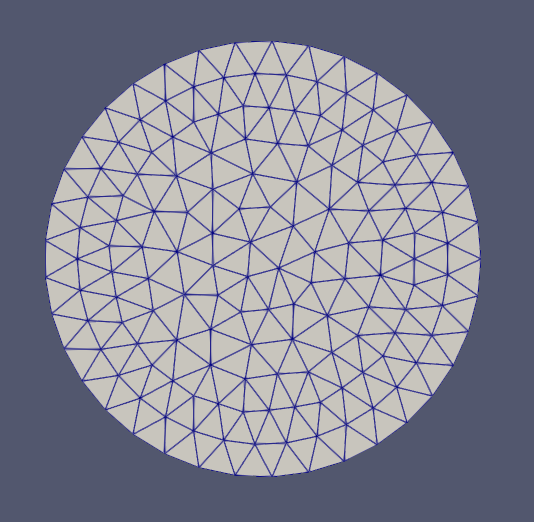
\includegraphics[width=\linewidth]{	processExample/circle.png}
	    \caption{Starting Mesh}
	\end{subfigure}
	\hspace*{\fill}	
	\begin{subfigure}{0.4\textwidth}
	    
\includegraphics[width=\linewidth]{	processExample/skin.png}	   
   	    \caption{Skinned Mesh}
	\end{subfigure}
	\caption{Top down view of a tri mesh. See how the only remaining elements after skinning \
	are the edge elements who had no neighbors.}
	\label{2DSkinExample}
\end{figure}

The skinning algorithm is implemented in the function \codeword{getSurfaceMesh()}, the source of which can be found in \codeword{surfaceMeshing.cpp}. Multiple overloads of this function exist that offer slight variations in functionality depending on the user requirements. These are documented on the Doxygen existing for this code[]. 


\subsection{Vacuum Generation}
\begin{figure}[ht]
	\begin{subfigure}{0.4\textwidth}
	    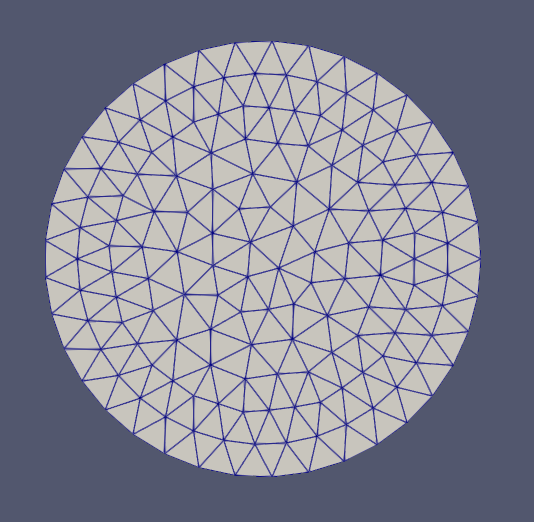
\includegraphics[width=\linewidth]{	processExample/circle.png}
	    \caption{Starting mesh.}
	\end{subfigure}
	\hspace*{\fill}	
	\begin{subfigure}{0.4\textwidth}
	    
\includegraphics[width=\linewidth]{	processExample/skin.png}
	    \caption{Skinned Mesh.}
	\end{subfigure}
	\vspace*{\fill}	
	\begin{subfigure}{0.4\textwidth}
	    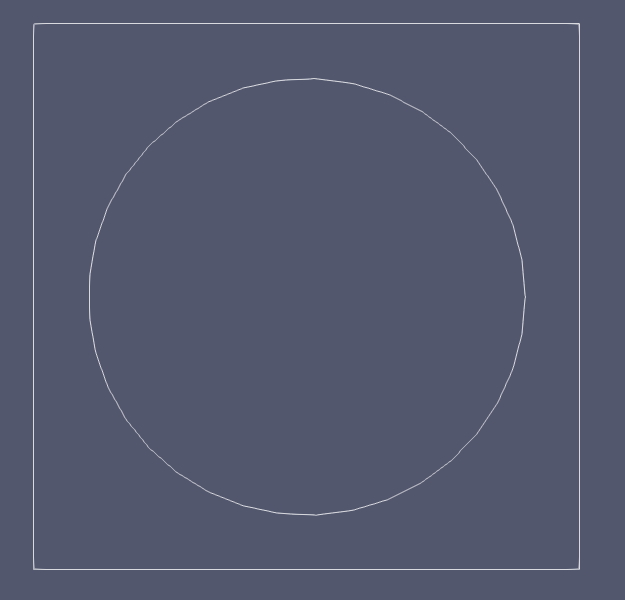
\includegraphics[width=\linewidth]{	processExample/bound.png}
	    \caption{Skinned mesh with boundary generated around it, and a seeding point in the middle of the circle.}
	    \label{SeedingPoint}
	\end{subfigure}
	\hspace*{\fill}	
	\begin{subfigure}{0.4\textwidth}
	    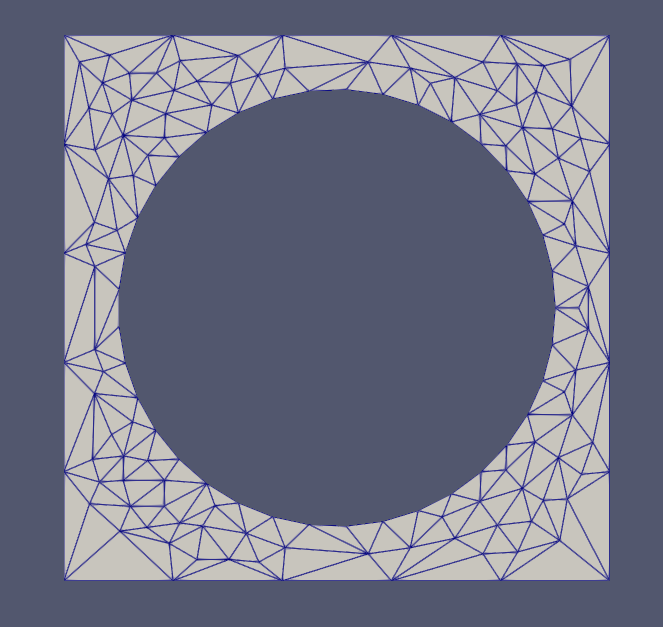
\includegraphics[width=\linewidth]{	processExample/vac.png}
	    \caption{Vacuum mesh generated in the space between the part and the boundary.}
	\end{subfigure}
	\caption{Example process of vacuum generation. This workflow should help\
	show why why the boundary mesh is necessary to generate the vacuum.}
	\label{Boundary Example}
\end{figure}
Vacuum generation is essentially a two step process; boundary generation, and tetrahedralisation. Boundary generation refers to the process of generating a boundary around the skinned mesh. Tetrahedralisation refers to the process of generating tetrahedra (or sometimes tri elements) in a well defined region. Boundary generation is necessary to define the space in which tetrahedralisation will occur. Figure \ref{Boundary Example} helps demonstrate this.

\subsubsection{Boundary Generation} \label{BoundaryGeneration}
To define a vacuum region in which tetrahedra can be generated, a boundary surrounding the skinned mesh must be created. Currently this tool only supports the generation of cubic boundaries. A cubic boundary should suffice for most problems however this functionality may be expanded in future to support the generation of other boundary types. Figure \ref{Boundary Example} helps demonstrate the need for a boundary mesh. However, unlike in Figure 2, most users will not be working with 2D planar geometry. It is more likely that a 3D mesh will be used, and henceforth a 3D boundary mesh is required. However, like the skin of a 3D part, this boundary mesh needs to be composed of 2D (tri) elements. Generating a cube composed of 2D mesh elements is easy in dedicated meshing software, but less trivial when you want to do it in your own code. Fortunately an aptly named C++ library, 'Triangle', exists that enables users to perform Delauny triangulation in the comfort of their own code. Even more fortunately, libIGL includes a wrapper around Triangle, making it easy to include. Triangle generates tri elements within planar 2D bounds. It is infact the tool used to generate the tri elements in the 2D example in Figure \ref{Boundary Example}.  Unfortunately, the functions within Triangle only take 2D coordinates (X and Y) as arguments. This is reasonable, given that creating planar geometry was likely what the library was written for. However, when trying to create a cube whose faces consist of tri mesh elements, clearly the coordinates for the nodes in this mesh need to exist in 3 dimensions. To generate a cube the same face is first generated 6 times. To allow this face to exist in 3D a column of zeroes is simply added to represent the z coordinate. This results in the generated face sitting on the XY (z=0) plane in 3D space.
\begin{figure}[ht!]
	\begin{subfigure}{0.4\textwidth}
		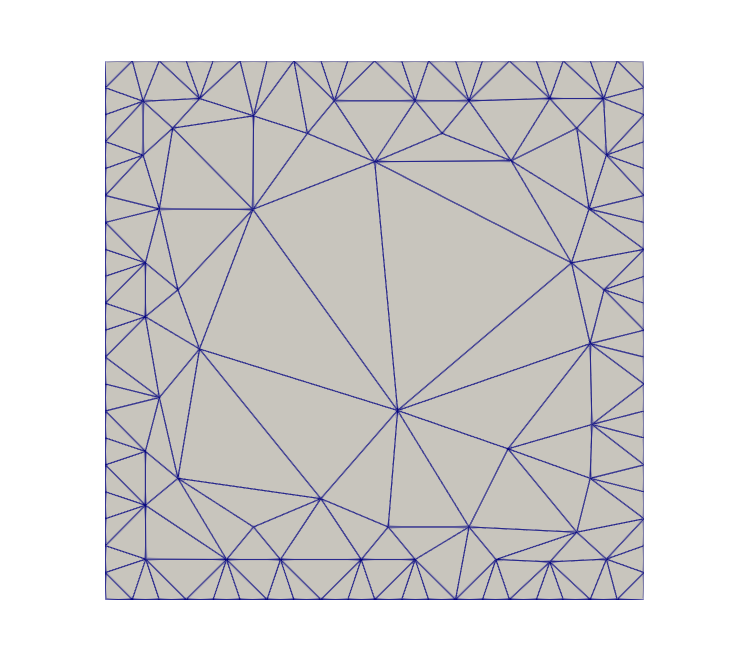
\includegraphics[width=\linewidth]{boundaryGen/square.png}
		\caption{Singular square face.}
	\end{subfigure}
	\hspace*{\fill}	
	\begin{subfigure}{0.4\textwidth}
		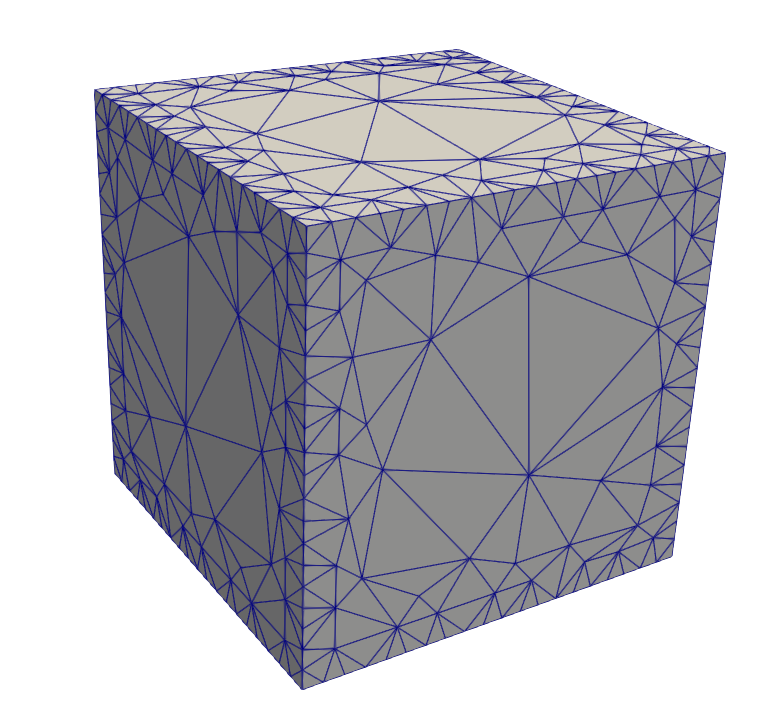
\includegraphics[width=\linewidth]{boundaryGen/cube.png}
		\caption{Duplicates of face transformed and combined, forming the cubic boundary.}
	\end{subfigure}	
	\caption{Example of boundary mesh generation.}
	\label{boundaryGenerationExample}
\end{figure}

Now that this face has 3D coordinates, it can be rotated and translated in 3D space. A face can be rotated by multiplying a selected rotation matrix by the nodal coordinates of all the nodes on that face. The connectivity data for the 2D elements will stay exactly the same, only the location of the nodes must be altered. Translation is achieved by adding/subtracting an offset to one of the 3 coordinates. Once the faces have been rotated/translated, they can be combined into one mesh, representing the boundary mesh. More information on how the meshes are combined can be found in Section \ref{rTree}. For now it should be made clear that this combination is particularly clean. The original meshed face has equidistant nodes on each edge, the number of which can be specified by the user. This means that when the faces are all combined there are guaranteed to be no hanging nodes.

The generation of a boundary around a coil is a case which has recieved some special attention in this tool. In some FE problems it is necessary for some of the faces of the coil to be coplanar with the vacuum boundary, as show in Figure \ref{coplanarCoilFig}. 

\begin{figure}
\begin{center}
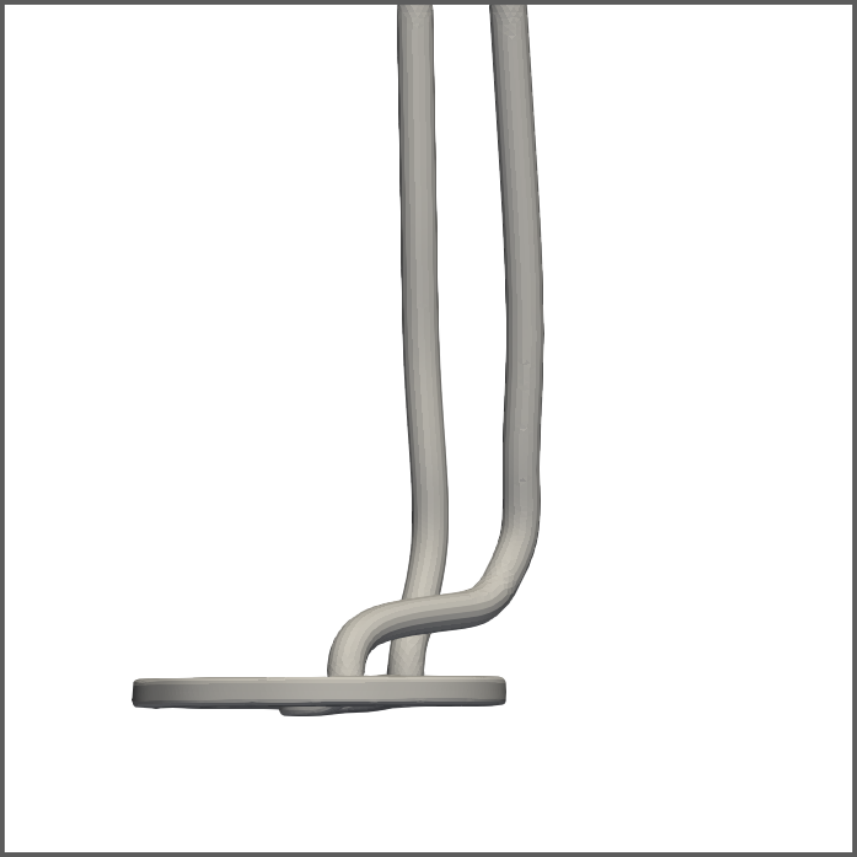
\includegraphics[width=0.5\linewidth]{coplanarCoil.png}
\end{center}
\caption{Example of how sometimes faces of the coil will be coplanar with boundary.}
\label{coplanarCoilFig}
\end{figure}

In this case it is not sufficient to just produce a cubic boundary, as combining the cubic boundary with the coil geometry will results in overlapping nodes and elements as shown in Figure \ref{coilBoundaryFix}. To solve this problem, one of the faces of the cubic boundary has to be produced with cutouts where the coplanar parts of the coil are. The elements and nodes on this boundary must also conform to those already existing on the coil. The other 5 faces of the cubic boundary are created as described prior, and then combined with the remaining one.

\begin{figure}[ht]
	\begin{subfigure}{0.48\textwidth}
		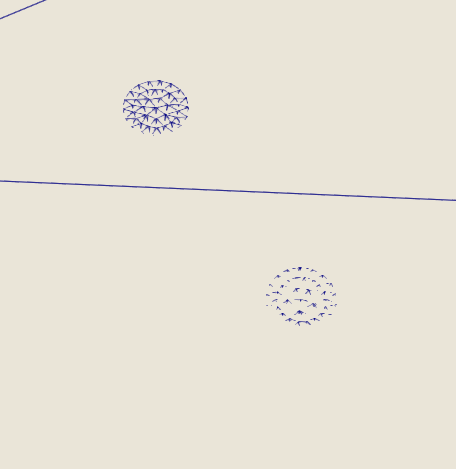
\includegraphics[width=\linewidth]{coplanarOverlap.png}
		\caption{Result when using standard boundary generation with coil faces being coplanar with boundary. Unusable mesh with overlapping elements}
	\end{subfigure}
	\hspace*{\fill}	
	\begin{subfigure}{0.48\textwidth}
		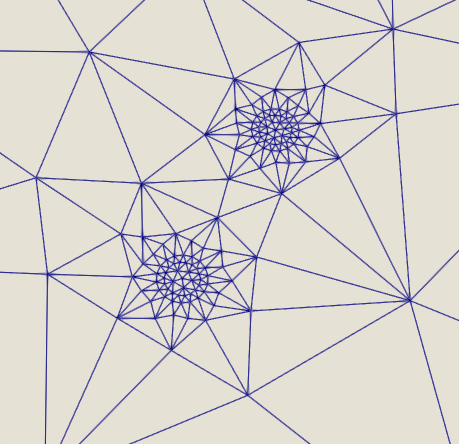
\includegraphics[width=\linewidth]{coplanarFixed.png}
		\caption{Correctly generated coil boundary, with the boundary elements conforming to those already existing on the coil.}
	\end{subfigure}	
	\caption{}
	\label{coilBoundaryFix}
\end{figure}


\subsubsection{Tetrahedralisation}
Tetrahedralisation refers to the process of generating tetrahedral mesh elements in the space described by the skinned mesh and the boundary mesh. The tool used to generate tetrahedra in this code is Tetgen. This is the tetrahedral analogue to the aforementioned Triangle library. Tetgen allows users to produce Delaunay tetrahedralizations of closed spaces. Tetgen includes many built it options that can be used to manipulate its behavoir. One of these options forces Tetgen to conform to the boundaries (skinned mesh and boundary mesh) input by the user. This makes it perfect for generating the vacuum mesh, as we can ensure the vacuum mesh conforms to the elements in the original mesh. 

Tetgen requires 4 main user inputs. The user must provide an input mesh, the coordinates of any "seeding points", any Tetgen options they wish to use, and data structures to store the output mesh. Tetgen can then generate tetrahedra in the defined vacuum region.But how does tetgen know not to generate tetrahedra within the skin of our original mesh? This is where seeding points come into use. Seeding points are points placed within any closed regions where users do NOT want any tetrahedra to be generated. Figure \ref{SeedingPoint} shows a seeding point placed in the middle of the closed region described by the circle mesh. This then prevents any elements being generated in the circle. However, not all meshes are as simple as a circle, and neccesitating prior knowledge of every closed region in the skinned mesh in order to add all the correct seeding points is unreasonable. Some complicated mesh geomatires may have 10's or 100's of internal closed regions. To automate the placement of seeding points, one seed point is placed for every 2D element of the skinned mesh. The coordinates of this point are calculated by taking the coordinated of the elements centroid, and taking a small step in the direction opposite to the outward pointing surface normal. The size of this "small step" is by default set to 1e-8, but can be specified using the command line options shown in Section \ref{CLFlags}. I have not found any problems with this method so far, but that does not mean it is perfect by any means. 

\subsection{Full Mesh Generation}
\subsubsection{Combining Meshes} \label{rTree}
Once a vacuum mesh has been generated, in most cases it needs to be recombined with the mesh of the original mesh. This presents a problem, as duplicate nodes will exist between the vacuum mesh and the original mesh. There exists a need therefore to locate the duplicate nodes so that one of the duplicates can be removed. With smaller meshes it would be feasible to run a node comparison between each node of each mesh. However, when larger meshes are used, this method becomes infeasible due to the $O(N^2)$ order of the node comparison. To avoid this issue, an r-Tree data structure is used to store all of the nodal coordinates of one of the meshes. Then the nodes in the second mesh can be used to query the r-Tree. If the query results in "no hits" (no results), then the node is not a duplicate and can be added to the final mesh. If any hits are found, then this node must be a duplicate, and it is not added to the final mesh. This operation is $O(nLog(n))$, resulting in much improved performance. In the examples included in the repo, all of the nodes of the original part are added to the r-Tree and the nodes of the vacuum mesh are used to query the r-Tree.

If a mesh consisted of only nodes, then this operation would be sufficient to combine two meshes. This is not the case however, as elements need to be considered. When a duplicate node is found, we prevent it being added to the final mesh. The elements in the second mesh need their connectivity data updated therefore, as they will still be looking for a node with an ID that matches that of the node not added. To fix this issue an std::map is used to keep a mapping of duplicate node ID's. The ID of the node not added to the mesh maps to its corresponding duplicate that exists in the mesh. To prevent the problem of adding nodes with unique positions, but non-unique node ID's, an offset is given to the nodes being placed into the mesh (i.e. the nodes from the Vacuum). This offset is equal the the largest node ID that exists in the original part mesh. This will ensure that no two nodes are given the same ID.

\subsubsection{Sidesets}
In problems that require a vacuum mesh, it is common that the mesh of the part will have some kind of radiative condition to the vacuum. Therefore it may be necessary to create a sideset in that represents the boundary of the original mesh. Thankfully, we know exactly which nodes/elements this sideset needs to contain; those that exist on the skin of the original mesh. This is fairly evident looking at Figure \ref{Boundary Example}, as clearly the boundary of the circle is its skin. Given this information it is trivial to create this sideset. When skinning the mesh, the user can choose to provide a container as an argument, which stores the ID's of the nodes in the original mesh which compose the skin. This container can then be used as an argument in an overload of the "combineMeshes()" function, allowing it to correctly create a sideset that represents the boundary.

You may be wondering why the r-Tree search is necessary if we know which nodes are duplicated. This is a fair question. Unfortunately, even though we know the node ID's of the duplicate nodes on the original mesh

\section{Building}
To build the library and the examples, just run the commands shown in Figure \ref{buildCommands} within the main 'Libmesh\textendash Skinning' directory. For those unfamiliar with the CMake build process, this shouldn't cause too much stress. The first command is making a directory called "build", where all of our build files will go. Having all the build files in a seperate folder is useful, as if you need to rebuild you can simply delete this folder and rebuild, without having to go on a witch hunt for nomadic CMake files. The second command moves you into the newly created build directory, in which you run the last command. This calls the main CMakeList.txt file, and builds the library as well as the examples. One argument is required, LIBMESH\textendash DIR, which should point to your libmesh install folder. For those with a MOOSE install the directory you want to point to will probably be "\codeword{<wherever-moose-lives>/moose/libmesh/installed}".

\begin{figure}[ht]
\begin{lstlisting}[language=bash]

	mkdir build
	cd build/
	cmake -DLIBMESH_DIR=\
		<dir_where_your_libmesh_install_lives> ../
\end{lstlisting}
\caption{Build}
\label{buildCommands}
\end{figure}

\section{Using}
\subsection{Using the examples}
There are three examples built in to the repo. These examples utilise  the functionality found in the library to different extents, and should be enough for most users to do what they need.

\subsubsection{skinner}
The first example, the source of which can be found in problems/skinner.cpp, is an example of how to get the skin of a mesh. This example loads in an input mesh given by the user and utilises the function \codeword{getSurfaceMesh} to obtain the skin of the input mesh. This can be used with meshes composed of 2D or 3D elements. In the 2D case, the skinned mesh will be composed of 1D edge facets, representing the boundary of the 2D boundary. In the 3D case, the skinned mesh will be composed of 2D facets. 

\begin{figure}[ht]
	\begin{subfigure}{0.48\textwidth}
		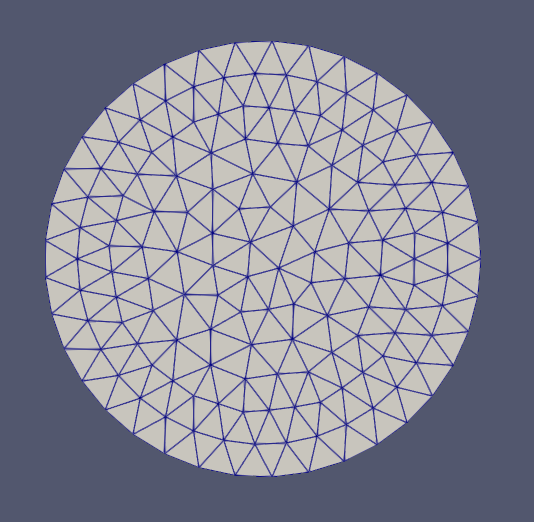
\includegraphics[width=\linewidth]{processExample/circle.png}
		\caption{Before}
	\end{subfigure}
	\hspace*{\fill}	
	\begin{subfigure}{0.48\textwidth}
		
\includegraphics[width=\linewidth]{processExample/skin.png}
		\caption{After}
	\end{subfigure}	
	\caption{Example of skinning a mesh composed of 2D facets.}
	\label{2DSkinningComp}
\end{figure}

For example, if you had a mesh called `myMesh.e`, from the command line you could enter 
\begin{lstlisting}[language=bash]
	./build/examples/skinner -i Meshes/myMesh.e
\end{lstlisting}
to skin a mesh called myMesh. This should successfully save a mesh called MyMesh\verb|_|skin.e in the directory where the command was called from. 

\subsubsection{generateVacuum}
The second example included in the repo is generateVacuum. Firstly the mesh is skinned, and then a cubic boundary is generated around it. The size of this boundary can be determined by CL flags documented in Section \ref{CLFlags}. If the user chooses not to provide a boundary size then a suitable size will be chosen by creating a bounding box around the input geometry. The largest dimension of this box is multiplied by a scaling factor to determine the size of the boundary. From here a list of seeding points is generated, and then the tetrahedralisation methods are called. Following successful tetrahedralisation, the mesh of the original part and the vacuum mesh are combined using the r-tree methods described in Section \ref{rTree}.

\subsection{generateCoilVacuum}
The third example program exists to help generate the vacuum mesh around a coil. This example specifically pertains to a coil which needs to have sidesets coincident with the vacuum mesh boundary. The example begins like the others, by skinning the coil mesh. To generate the boundary for the coil, the \codeword{generateCoilBoundary} method is called. This method is described in Section \ref{BoundaryGeneration}. Once the coil boundary is generated, the seeding points can be calculated and tetrahedralisation of the vacuum region can take place. 

For the process in \ref{BoundaryGeneration} to be successful, the \codeword{generateCoilBoundary} method needs to know which coil sidesets are coplanar with the vacuum boundary. By default, the function looks for sidesets called "coil\_in" and "coil\_out"

There is one notable restriction with this example. The coil sidesets that are coplanar with the boundary MUST exist on the same plane. Figure --- helps exemplify this limitation. Apologies, this functionality is not in yet.

\newpage

\subsection{Command Line Options} \label{CLFlags}
When using the examples, there a few command line flags that can be set by the user. Table \ref{CLFlagsTab} shows the available options, and a short description of what they do.

\begin{table}[ht!]
\begin{center}
\begin{tabularx}{0.9\textwidth}{
  | >{\raggedright\arraybackslash}X 
  | >{\raggedright\arraybackslash}X 
  | >{\raggedright\arraybackslash}X | }
  \hline
  \textbf{Option} & \textbf{Flag} & \textbf{Description} \\
  \hline
  \hline
  Input Mesh & -i, \texttt{-{}-}input & The mesh the user wants to use\\
  \hline
  Output Mesh & -o, \texttt{-{}-}output & Optional dir\\
  \hline 
  Max Tri Element Area & \texttt{-{}-}max\texttt{\_}tri & Maximum area constraint on triangles elements produced for the boundary\\
  \hline 
  Max Tet Element Volume & \texttt{-{}-}max\texttt{\_}tet & Maximum volume constraint on tet elements produced in the vacuum region\\
  \hline 
  Output Mesh & -o, \texttt{-{}-}output & Optional dir\\
  \hline
\end{tabularx}
\caption{Table listing command line switches accessable by users}
\label{CLFlagsTab}
\end{center}
\end{table}


\subsection{Using the library}
As previously mentioned, the functionality found in this repo is built into a library called "VacuumMeshing". The example executables are linked to this library in order to utilise the funtionality. There is no reason that this library couldn't be linked to any of your own projects. Within the repo, naviating to "./VacuumMeshing/CMakeLists.txt" will show you how the library is built. The libIGL libraries that are linked in when the library is created have PUBLIC "inheretence". This means that any targets depending on this library will automatically be linked in with the necessary libIGL libs. This saves the user (you) having to mess around with ligIGL includes/libs. The MPI lib linked in with the library is set as PRIVATE, so that when building your own projects they will NOT link against the MPI version used to build the VacuumMeshing library.

\subsection{Extras}
Doxygen...

\end{document}
